\subsection*{Aufgabe 2 - Bestimmung der Bewegungsgleichung}

\subsubsection*{Generalisierte Koordinaten}
Die Wahl fällt zu $y(1) = \alpha$ und $y(2) = \beta$. Die generalisierten Koordinaten sind somit die Winkel der Gelenke 2 und 3.

\subsubsection*{Lagrang'sche Gleichung 2. Art}
Die Bewegungsgleichung des Arms kann mit folgender Gleichung beschrieben werden:

\begin{equation}
	M(y) \cdot \ddot{y} + D(y,\dot{y}) \cdot \dot{y} + g(y) = \tau_{Reib} + \tau_{Aktormoment}
\end{equation}

Dabei berechnet sich die Massenmatrix $M_{i}$ mit $M = \sum_{i}{M_{i}}$ von Arm i nach:
\begin{equation}
	M_{i}(y) = \left[m_{i}J_{TiS}^{T}(y) \cdot J_{TiS}(y) + 
	J_{RiS}^{T}(y) \cdot S_{0,iS}(y) \cdot I_{iS,iS} \cdot S_{0,is}^{T}(y) J_{RiS}(y) \right]
\end{equation}

Dabei sind $J_{TiS}(y)$ und $J_{RiS}(y)$ die Jakobimatrizen für den Schwerpunkt für Körper 
i der Translation beziehungsweise Rotation und $I_{iS,iS}$
der Trägheitstensor von Körper i dargestellt in dessen Schwerpunkt.

Mithilfe der Transformationsmatrix $S_{0,iS}(y)$ kann der Trägheitstensor im Inertialsystem dargestellt werden:
\begin{equation}
	I_{iS,0} = S_{0,iS}(y) \cdot I_{iS,iS} \cdot S_{0,is}^{T}(y)
\end{equation}


Für  $D(y,\dot{y})$ gilt:
\begin{equation}
	D_{kj} = \sum_{i=1}^{n}h_{ijk}(y)\dot{y}_{i}
\end{equation}
mit den Christoffel-Symbolen
\begin{equation}
	h_{ijk} = \frac{1}{2}\left(	\frac{\partial M_{kj}}{\partial y_{i}} + 
								\frac{\partial M_{ki}}{\partial y_{j }} -
								\frac{\partial M_{ij}}{\partial y_{k}}				\right)
\end{equation}

Der Graviationsvektor $g(y)$ ist definiert als
\begin{equation}
	g(y) = \left[ 
			\frac{\partial{V}}{\partial{y_{1}}} , 
			\frac{\partial{V}}{\partial{y_{2}}}
	\right]
\end{equation}

mit der potentiellen Energie $V$:
\begin{equation}
	V(y) = \sum_{i}V_{i} = \sum_{i}m_{i}g \cdot p_{iS,0}(y) 
\end{equation}
nach 2.1.11 Lagrange'sche Gleichungen zweiter Art in \cite{Fehr23}.
Die Umsetzung der genannten Gleichungen wurde mit der Symbolic Math Toolbox in Matlab implementiert.
Gleichung (1) liefert dann jeweils eine Differentialgeichung pro generalisierte Koordinaten $y_{i}$.



\subsubsection*{Reibungsterm}
In Gleichung (1) geht das Reibmoment der Lagerung der Arme $\tau_{Reib}$ mit ein:
\begin{figure}[H]
	\centering
	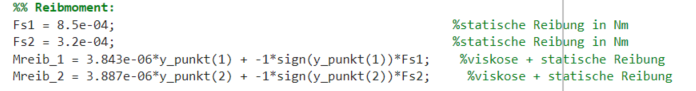
\includegraphics[width=0.95\textwidth]{Reibung.png}
	\caption{Modellierung der Lagerreibung}
\end{figure}
